\newpage 
\section{Spatially Continuous Material Properties} \label{s2}

This section provides the theoretical background for Monte Carlo (MC) coupled multi-physics simulations with spatially continuous materials. Section \ref{sec21} explains the theory behind Functional Expansion Tally (FET), followed by the calculation of the polynomial basis required for FET in section \ref{sec22} and how to overcome function discontinuities in section \ref{sec22x}. The variance estimation of the reconstructed power is briefly discussed in section \ref{sec22a}. The use of delta-tracking for spatially continuous materials is described in section \ref{sec23}, along with the computation of majorant cross-sections in section \ref{sec24}. Finally, section \ref{sec25} summarizes the calculation flow for MC coupled multi-physics simulations with spatially continuous materials.

\subsection{Functional Expansion Tally} \label{sec21}

In the FET methodology \cite{gries, ellis}, the actual power shape solution is approximated through a truncated linear combination of polynomials, with MC tallies used to calculate the coefficients of these polynomials. Therefore, the spatially continuous power distribution can be approximated using FET by expanding the tally quantity into a linear combination of polynomials $\psi(\vec{\xi})$, as shown below:
\begin{equation}
    f\left(\vec{\xi}\right)=\sum_{n=0}^{\infty}{{\bar{a}}_nk_n\psi_n\left(\vec{\xi}\right)},
    \label{eq1}
\end{equation}
\begin{equation}
    {\bar{a}}_n=\left\langle f,\psi_n\right\rangle=\int_{\Gamma}{f\left(\vec{\xi}\right)\psi_n\left(\vec{\xi}\right)\rho\left(\vec{\xi}\right)d\vec{\xi}\ }.
    \label{eq2}
\end{equation}
Here, ${\bar{a}}_n$ represents the expansion coefficients, $\vec{\xi}$ denotes the neutron phase space comprising $\left(\vec{r},\hat{\mathrm{\Omega}},E\right)$, and $k_n$ is the normalization constant, which can be determined based on the chosen polynomial basis set that can be expressed as:
\begin{equation}
    k_n=\frac{1}{||\psi_n||^2},
\end{equation}
where
\begin{equation}
    ||\psi_n||^2=\int_{\Gamma}{\psi_n^2\left(\vec{\xi}\right)\rho\left(\vec{\xi}\right)d}\vec{\xi}\ .
    \label{eq4}
\end{equation}
Lastly, the $\rho\left(\vec{\xi}\right)$ is the weighting function that shall be both complete and orthogonal with respect to $\psi_n\left(\vec{\xi}\right)$.

Fortunately, the integrals required to obtain the expansion coefficients in Eq. \ref{eq2} can be easily calculated in MC simulations using both analog and collision-based estimators. The unbiased collision-based estimator for the coefficients ${\bar{a}}_n$, used to reconstruct the power (as per Eq. \ref{eq1}), is defined as:
\begin{equation}
    {\bar{a}}_n=\frac{1}{N}\sum_{i=1}^{N}{\sum_{k=1}^{K_i}{w_{i,k}\frac{\kappa\left({\vec{\xi}}_{i,k}\right)}{\Sigma_t\left({\vec{\xi}}_{i,k}\right)}}\psi_n\left({\vec{\xi}}_{i,k}\right)\rho\left({\vec{\xi}}_{i,k}\right)}.
    \label{eq5}
\end{equation}
In Eq. \ref{eq5}, $N$ represents the total number of particles in each batch, $K_i$ is the total number of collisions for particle $i$, $w_{i,k}$ is the weight of particle $i$ at collision $k$, $\kappa\left({\vec{\xi}}_{i,k}\right)$ is the energy released per fission at the phase space point ${\vec{\xi}}_{i,k}$, and $\mathrm{\Sigma}_\mathrm{t}\left({\vec{\xi}}_{i,k}\right)$ is the total macroscopic cross section at the phase space point ${\vec{\xi}}_{i,k}$.

While any polynomial basis can be used, a set of orthogonal polynomials is generally preferred. By choosing the weighting function $\rho\left(\vec{\xi}\right)$ as the zeroth order of an orthogonal polynomial set, which equals unity, Eq. \ref{eq4} and Eq. \ref{eq5} can be simplified.

FET implementation often assumes that the solutions are separable. For instance, in cylindrical geometry, the solution is assumed to be separable as:
\begin{equation}
f\left(r,\theta,z\right)=g\left(r,\theta\right)h\left(z\right).
\end{equation}
This separability offers two key advantages: (1) it significantly reduces memory requirements, especially for large core problems involving Xenon feedback, and (2) it improves particle tracking efficiency by reducing the number of coefficients that need to be tallied. Numerical experiments have demonstrated that separable FET provides a reasonable approximation for non-separable distributions, achieving this at a fraction of the computational cost compared to the fully coupled solution \cite{gries}.

\subsection{Polynomials Calculation} \label{sec22}

As discussed earlier, although any polynomial basis can be used, a set of orthogonal polynomials is generally preferred. In reactor calculations, Legendre and Zernike polynomials are most commonly used. Legendre polynomials serve as the basis for approximating functions in rectangular geometries, while Zernike polynomials are used for cylindrical geometries, such as fuel pellets.

The construction of Legendre polynomials can be done recursively as given by:
\begin{equation}
    P_n\left(x\right)=\frac{\left(2n-1\right)xP_{n-1}\left(x\right)-\left(n-1\right)P_{n-2}\left(x\right)}{n},
\end{equation}
with $P_0=1$ and $P_1=x$. Note that when constructing both Legendre and Zernike polynomials, the variable must be scaled into its domain. For example, the Legendre polynomials' variable $x$ must be scaled over the interval $[-1, 1]$. Therefore, if Legendre polynomials need to be calculated across the axial direction of an active reactor core, for instance, from 11.951 cm to 377.711 cm, the variable $x$ in the range $[11.951, 377.711]$ must be scaled to the range $[-1, 1]$.

Zernike polynomials form an orthogonal set of polynomials defined on a unit disk with variable domain of $[0, 1]$. They have traditionally been widely applied in optics, particularly in wavefront analysis due to their ability to represent circularly symmetric functions efficiently. To provide a better illustration on the Zernike polynomials, the first four orders of Zernike polynomials are plotted in Figure \ref{fig_21}. Note that, in Figure \ref{fig_21}, the Zernike polynomials of order $Z_n^0$ have a uniform profile across the azimuthal direction.

\begin{figure}
    \centering
    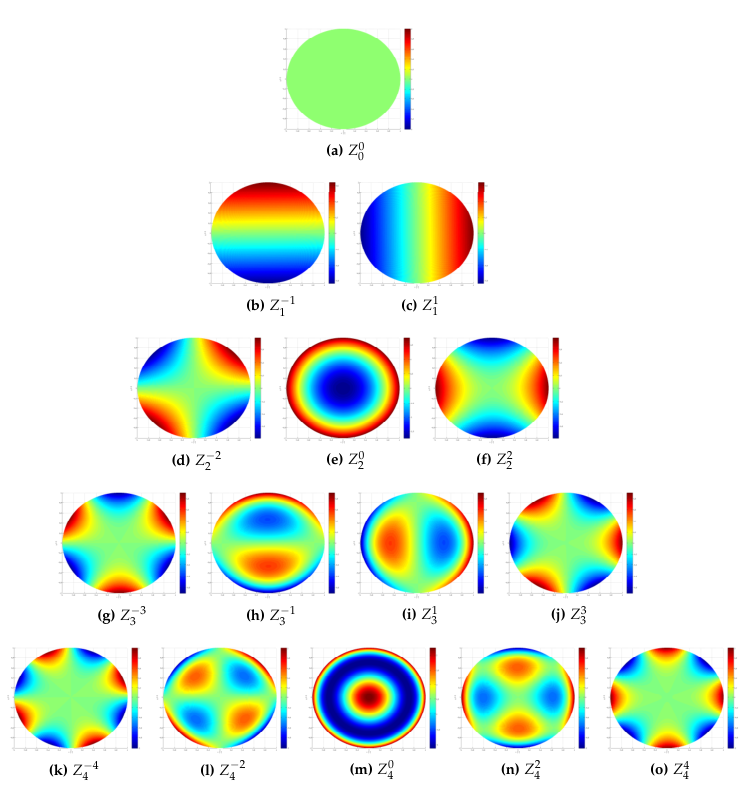
\includegraphics[width=0.8\textwidth]{figs/zernike.png}
    \caption[Zernike polynomial orders zero through four]{Zernike polynomial orders zero through four. Adapted from \cite{ellis}}
    \label{fig_21}
\end{figure}

The radial components of Zernike polynomials are conventionally calculated using the general equation as shown in Eq. \ref{eq6}.
\begin{equation}
R_n^m(r) = \sum_{s=0}^{\frac{n-m}{2}} (-1)^s \frac{(n-s)!}{s! \left( \frac{n+m}{2} - s \right)! \left( \frac{n-m}{2} - s \right)!} r^{n-2s}
\label{eq6}
\end{equation}
In this work, however, we introduce a highly efficient method for constructing the radial components of Zernike polynomials for FET. This approach is based on the recursive technique described in \cite{honarvar}, where the radial components are calculated through the following relation:
\begin{equation}
    R_n^m\left(r\right)=r\left[R_{n-1}^{\left|m-1\right|}\left(r\right)+R_{n-1}^{m+1}\left(r\right)\right]-R_{n-2}^m\left(r\right)\ .
    \label{eq7}
\end{equation}
In this way, $R_0^0$, $R_2^0$, $R_3^1$, and $R_n^m$ for $n=m$ can be determined manually as shown in Eq. \ref{eq7a}, then followed by the computation of the rest radial components using Eq. \ref{eq7}.
\begin{equation}
    \begin{split}
    R_0^0(r) &= 1, \\
    R_2^0(r) &= 2r^2-1, \\
    R_3^1(r) &= 3r^3-2r, \\
    R_n^m(r) &= r^n \text{ for } n = m.
    \end{split}
    \label{eq7a}
\end{equation}

Table \ref{tab_z} presents a comparison of the CPU time required to calculate the radial components of the Zernike polynomials a million times using Eq. \ref{eq7} and Eq. \ref{eq6}. As indicated in the table, Eq. \ref{eq7} provides a more efficient approach for calculating the radial components of Zernike polynomials, particularly at higher orders. This increased efficiency is attributed to its recursive nature, which reduces the number of mathematical operations compared to the conventional method in Eq. \ref{eq6}. This implementation of Zernike polynomial computation represents the first application of this method in FET for reactor core simulations.

\begin{table}
    \centering
    \caption[CPU time for calculating the radial components of the Zernike polynomials]{CPU time for calculating the radial components of the Zernike polynomials a million times.}
    \label{tab_z} 
    % \begin{adjustbox}{width=0.6\textwidth} % Adjust your table to the text width
    \begin{tabular}{| c | c | c | c | }
    \hline
           & \multicolumn{2}{c|}{CPU time (seconds)} &        \\
    \cline{2-3}
     Order & Equation \ref{eq7} & Equation \ref{eq6} & Speedup \\
     \hline
     5    & 0.0252  & 0.1179 & 4.7      \\ \hline
     10   & 0.0702  & 0.6236 & 8.8      \\ \hline
     15   & 0.1450  & 2.3122 & 15.9     \\ \hline
     20   & 0.2292  & 8.4591 & 36.9     \\ \hline
    \end{tabular}
    % \end{adjustbox}
\end{table}

Finally, once these radial components are established, the complete Zernike polynomials $Z_n^m$ can be calculated as follow:
\begin{equation}
Z_n^m(r,\theta) = 
\begin{cases} 
    R_n^m \cos (m\theta) & \text{if } m > 0, \\
    R_n^m \sin (m\theta) & \text{if } m < 0, \\
    R_n^m                & \text{if } m = 0.
\end{cases}
\end{equation}
However, for MC multi-physics applications in this study, the constructions the radial components for $m=0$ only are sufficient under the assumption that power variation within the fuel pellet occurs predominantly along the radial direction, with uniformity along the azimuthal direction.

\subsection{Overcoming Discontinuities} \label{sec22x}
One limitation of the FET method is that its polynomials are primarily effective for approximating smooth distributions, with accuracy decreasing when applied to functions with discontinuities, such as those found in the axial power profile due to the presence of spacer grids. As proposed by Griesheimer \cite{gries}, this issue can be mitigated by using a piecewise expansion. In this approach, a tally region with known discontinuities is divided into two or more smaller regions, each expected to have a continuous solution, resulting in more accurate approximations.

\begin{figure}
    \centering
    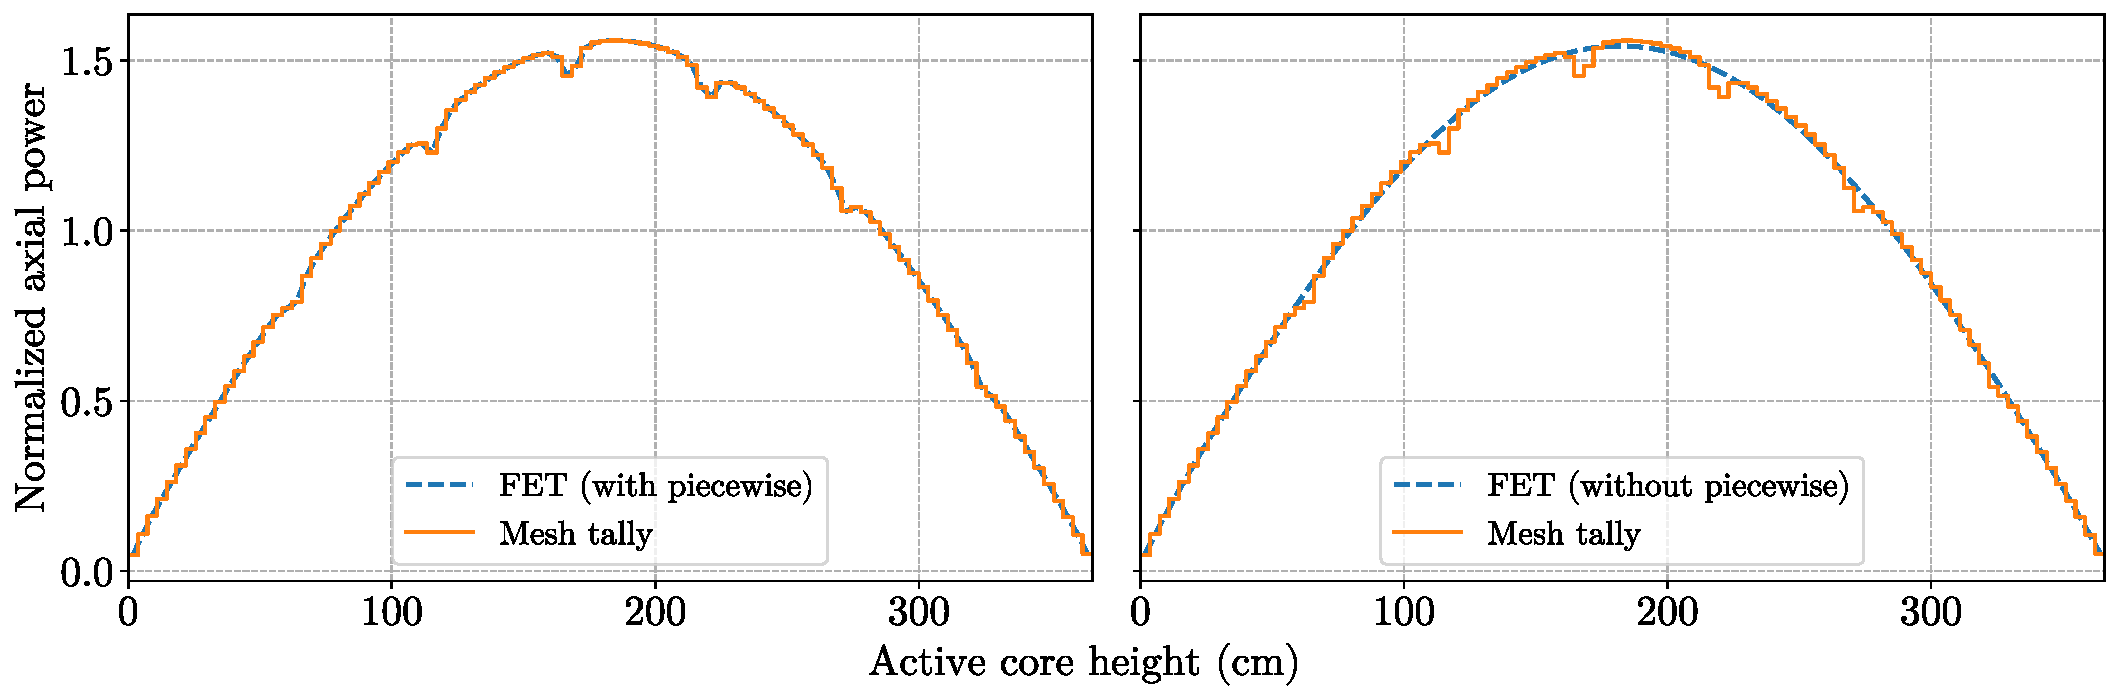
\includegraphics[width=1.0\textwidth]{figs/axi_pow_comparison.pdf}
    \caption[Comparisons of axial power from mesh tally and FET.]{Comparisons of axial power from mesh tally and FET, both with and without the use of piecewise expansions. Both FET cases uses 8\textsuperscript{th} order Legendre polynomials expansions.}
    \label{fig_21x}
\end{figure}

Figure \ref{fig_21x} shows the comparisons of axial power from mesh tally and FET, both with and without the use of piecewise expansions. The FET cases in the figure utilize 8\textsuperscript{th} order Legendre polynomial expansions. As demonstrated, the axial power depression due to the presence of spatial grids cannot be accurately modeled using a single expansion, and higher-order Legendre polynomials do not resolve the inaccuracies near power depression areas. As observed in Figure \ref{fig_21y}, even a 12\textsuperscript{th} order expansion does not accurately capture the power depressions in axial power. Conversely, with piecewise expansions, even a 6\textsuperscript{th} order expansion can accurately model these depressions as can be seen in the Figure \ref{fig_21z}.

\begin{figure}
    \centering
    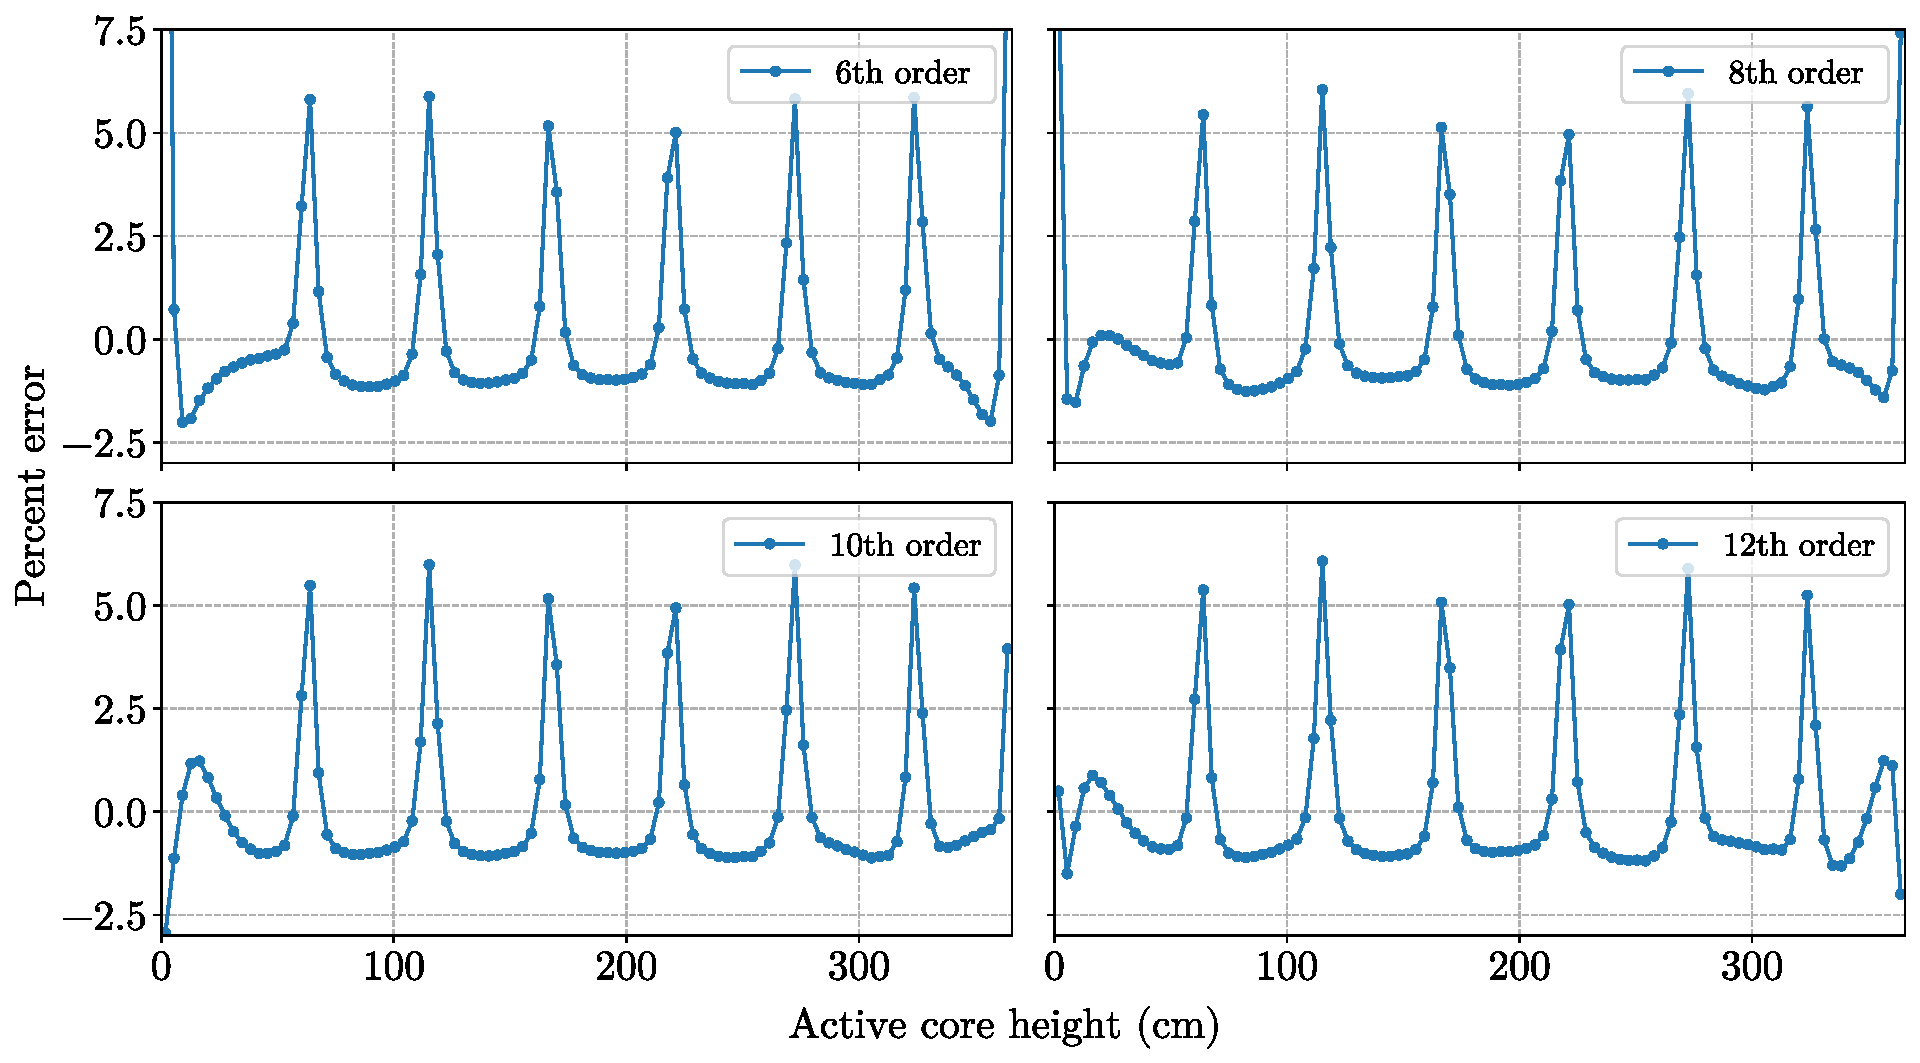
\includegraphics[width=0.88\textwidth]{figs/no_piecewise.pdf}
    \caption[Percent error in axial power from FET without the use of piecewise expansions.]{Percent error in axial power from FET without the use of piecewise expansions for 6\textsuperscript{th}, 8\textsuperscript{th}, 10\textsuperscript{th}, and 12\textsuperscript{th} order expansions.}
    \label{fig_21y}
\end{figure}

\begin{figure}
    \centering
    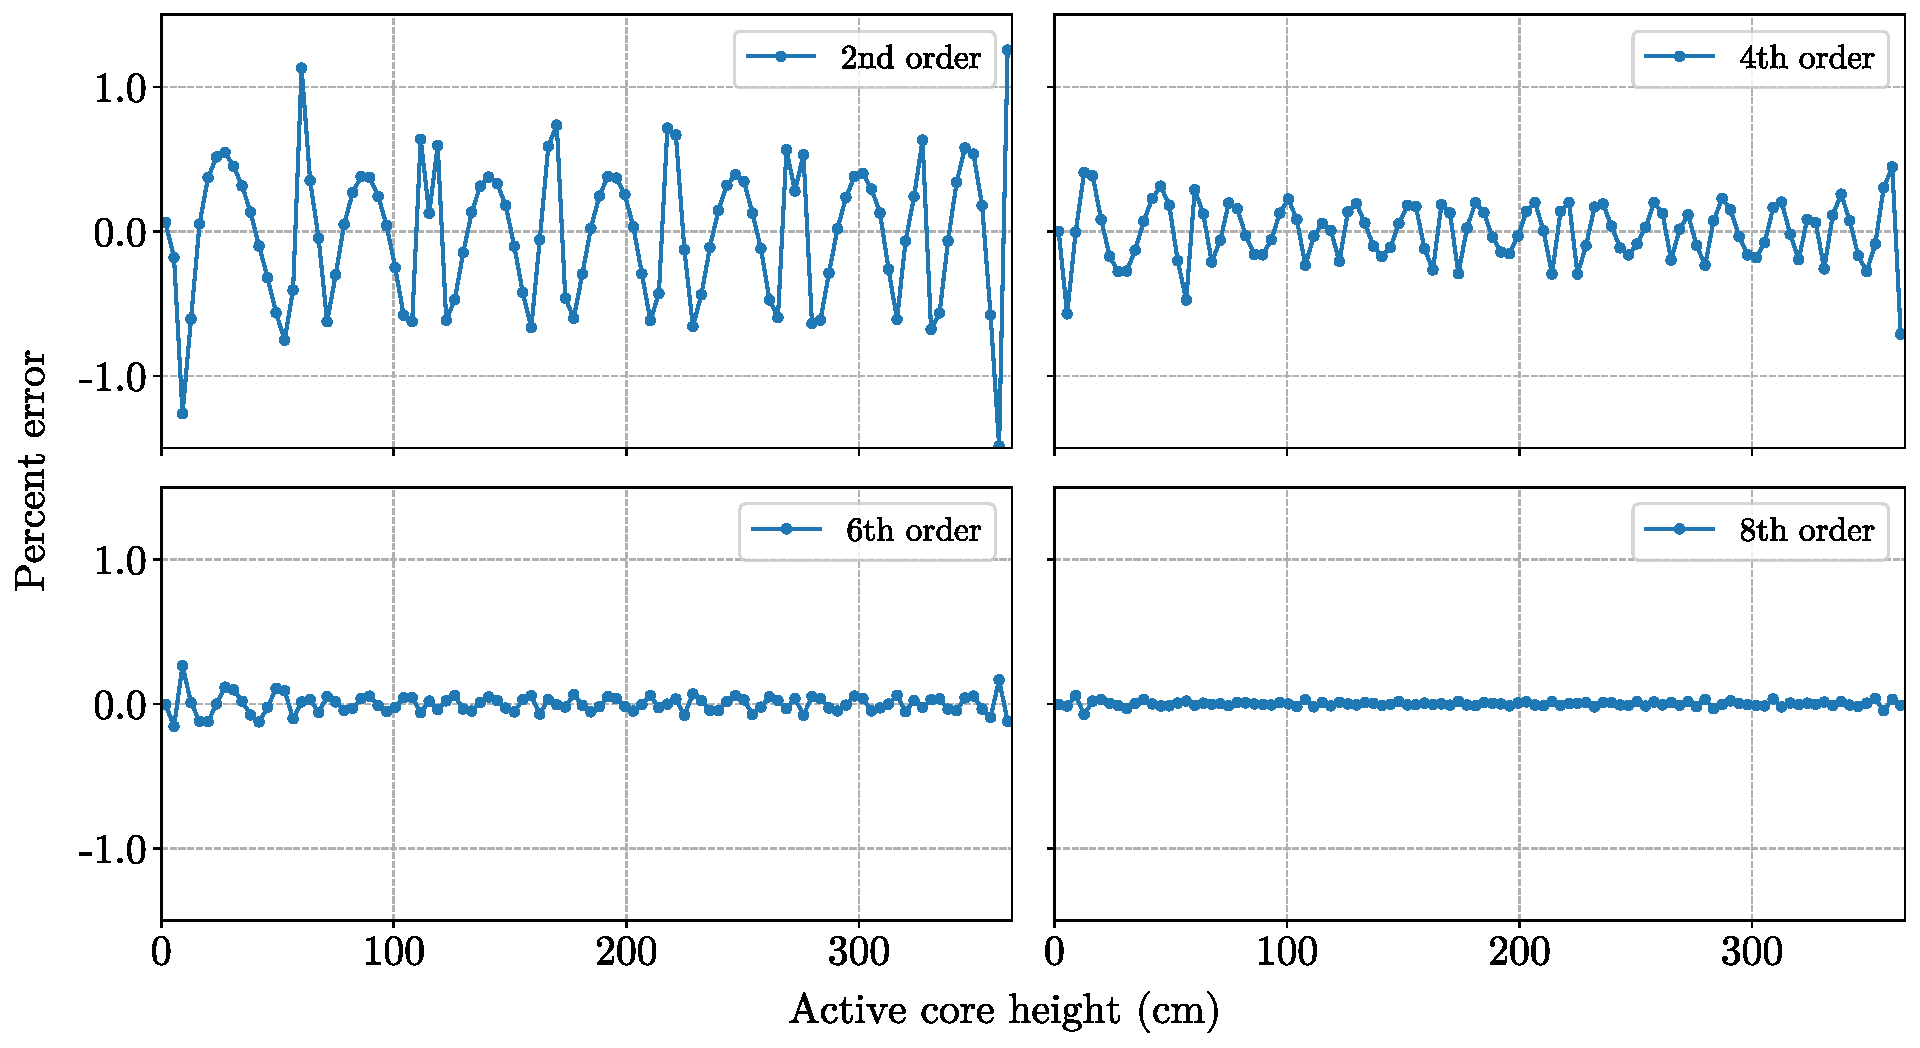
\includegraphics[width=0.88\textwidth]{figs/piecewise.pdf}
    \caption[Percent error in axial power from FET with the use of piecewise expansions.]{Percent error in axial power from FET with the use of piecewise expansions for 2\textsuperscript{nd}, 4\textsuperscript{th}, 6\textsuperscript{th}, and 8\textsuperscript{th} order expansions.}
    \label{fig_21z}
\end{figure}

However, employing piecewise expansions comes with a cost. The use piecewise expansions require more number expansion coefficients that must be stored because each segmented expansion has its own set expansion coefficients. For instance, in the Watts Bar reactors which have seven spacer grids, the number of 8\textsuperscript{th} order Legendre expansion coefficients that must be stored with the use of piecewise expansion is 126 coefficients compared to only 9 coefficients if single expansion is used. Fortunately, as will be shown later, the overall memory savings from utilizing FET are substantial compared to conventional cell tallies in multi-physics simulations.

\subsection{Variance Estimation}\label{sec22a}

Variance estimation is an integral part in the MC simulations, as lower variance increases confidence in the results. In the implementation of FET in this study, although FET coefficients are tallied during particle tracking, their variances are not directly calculated. Instead, the variances of the reconstructed tallies are computed, as the primary goal of the calculations is not the coefficients themselves but the reconstructed tallies, such as power and reaction rates. The estimated variances for the reconstructed tallies from FET are calculated in a similar manner to traditionally tallied quantities in MC simulations.

\subsection{Delta-tracking} \label{sec23}
Due to the continuous variation of material properties across the fuel pin, delta-tracking is employed as an alternative to conventional surface-tracking. Surface-tracking is not suitable in a continuous medium because the distance to collision is sampled using the following equation:
\begin{equation}
    s = -\frac{\ln(\xi)}{\Sigma_{t}(E)},
    \label{eq8}
\end{equation}
which assumes a spatially constant total cross-section $\Sigma_{t}(E)$. If the total cross-section changes during the neutron's random walk, the particle track must be terminated, and a new distance to collision recalculated. Unlike conventional surface-tracking, delta-tracking allows the neutron's random walk to continue through multiple material regions without needing to terminate the particle track at each boundary surface where the change in total cross-section takes place.

Delta-tracking, as described in \cite{leppanen_2017, woodcock}, makes the total interaction probability uniform in all cells, regardless of their material properties, by introducing majorant cross-sections. This allows for the uniform sampling of the distance to collision as given by:
\begin{equation}
    s = -\frac{\ln{\left(\xi\right)}}{\Sigma_{maj}(E)},
    \label{eq8}
\end{equation}
where \(\xi\) is a uniformly distributed random variable on the interval \([0,1]\), and \(\Sigma_{maj}(E)\) is the majorant cross-section which will be explained later. In this study, to improve rejection sampling efficiency, the interaction probability is made uniform only within the delta-tracking region, which is typically defined at the assembly level. 

To preserve the physical nature of neutron transport while allowing the neutron random walk to continue through multiple material regions, the interaction probability in each material is adjusted by introducing virtual collisions. These are rejected collisions based on the total cross section at the neutron's collision site. In practice, this involves rejection sampling, where the collision is only accepted as a physical collision with the probability:

\begin{equation}
    p = \frac{\Sigma_t(\vec{r},E)}{\Sigma_{maj}(E)}.
    \label{eq9}
\end{equation}

If the probability $p$ obtained in Eq. \ref{eq9} is smaller than the newly sampled random number $\xi$, the collision is rejected as virtual. In this case, a new distance to collision is sampled using Eq. \ref{eq8}, and the neutron random walk is continued. Conversely, if $p \geq \xi$, the collision is accepted as a physical collision, where the actual neutron interaction is simulated and the tally is performed.

Although the value of the majorant cross-section can be chosen arbitrarily, setting it too high can reduce the efficiency of the rejection sampling procedure. Therefore, it is common practice to choose the majorant cross-section as:
\begin{equation}
    \Sigma_{maj}(E) = \max{\left[\Sigma_t(\vec{r},E)\right]}.
    \label{eq10}
\end{equation}
This ensures that the rejection sampling remains efficient while maintaining the physical nature of the particle tracking.

The delta-tracking has a drawback in geometries with significant material heterogeneity, where the total cross sections of different materials vary considerably \cite{leppanen_2010}. A common example is a LWR fuel assembly containing localized heavy absorbers, such as control rods or burnable absorber pins. In these cases, the absorber's cross section dominates the majorant at low energy, even though it occupies only a small portion of the total volume. This leads to a low probability of sampling a physical collision in regions outside the absorber. The impact of localized high absorbers, as commonly found in LWR problems, on the computational speed will be evaluated in subsection \ref{sec41}.

\subsection{Majorant cross-section Computation} \label{sec24}

One of the main challenges in the delta-tracking for spatially continuous material properties is specifying the majorant cross-section (XS). The continuous distributions of fuel temperature, coolant density, and boron nuclide density significantly influence the XS across the delta-tracking region. Since each nuclide has different energy grids, the majorant XS is stored energy-wise in uniform majorant energy bins (MEB). Each MEB contains one or more energy grids of the point-wise XS in the MC cross-section library.

The calculation of the majorant XS begins by identifying the maximum microscopic total XS within a given MEB for different temperatures. Figure \ref{fig_2} compares the majorant microscopic XS of U-238 across a temperature range of 500 K to 1400 K with the point-wise microscopic XS of U-238 at 700 K. Once the majorant microscopic XSs for each nuclide are determined, they are multiplied by the corresponding highest possible nuclide densities within a given material to obtain the material-wise majorant XS. Finally, the majorant XS for each MEB is determined by selecting the maximum material-wise majorant XS within that MEB, as illustrated in Figure \ref{fig_3}.

Numerical experiments suggest that the ideal number of MEBs is 1,200 which distributed across thermal, resonance, and fast regions. If the number of MEBs is too small, rejection sampling becomes inefficient. Conversely, if too many MEBs are used, there is a higher likelihood of underestimating the majorant XS, where it may fall below the actual total XS of the material where the neutron collision occurs. To mitigate this, the maximum total XS is searched for within overlapping MEBs to ensure the largest macroscopic XS is captured for a given energy bin. By optimizing the number of MEBs and using overlapping MEBs, the probability of underestimating the majorant XS can be minimized.

\begin{figure}
    \centering
    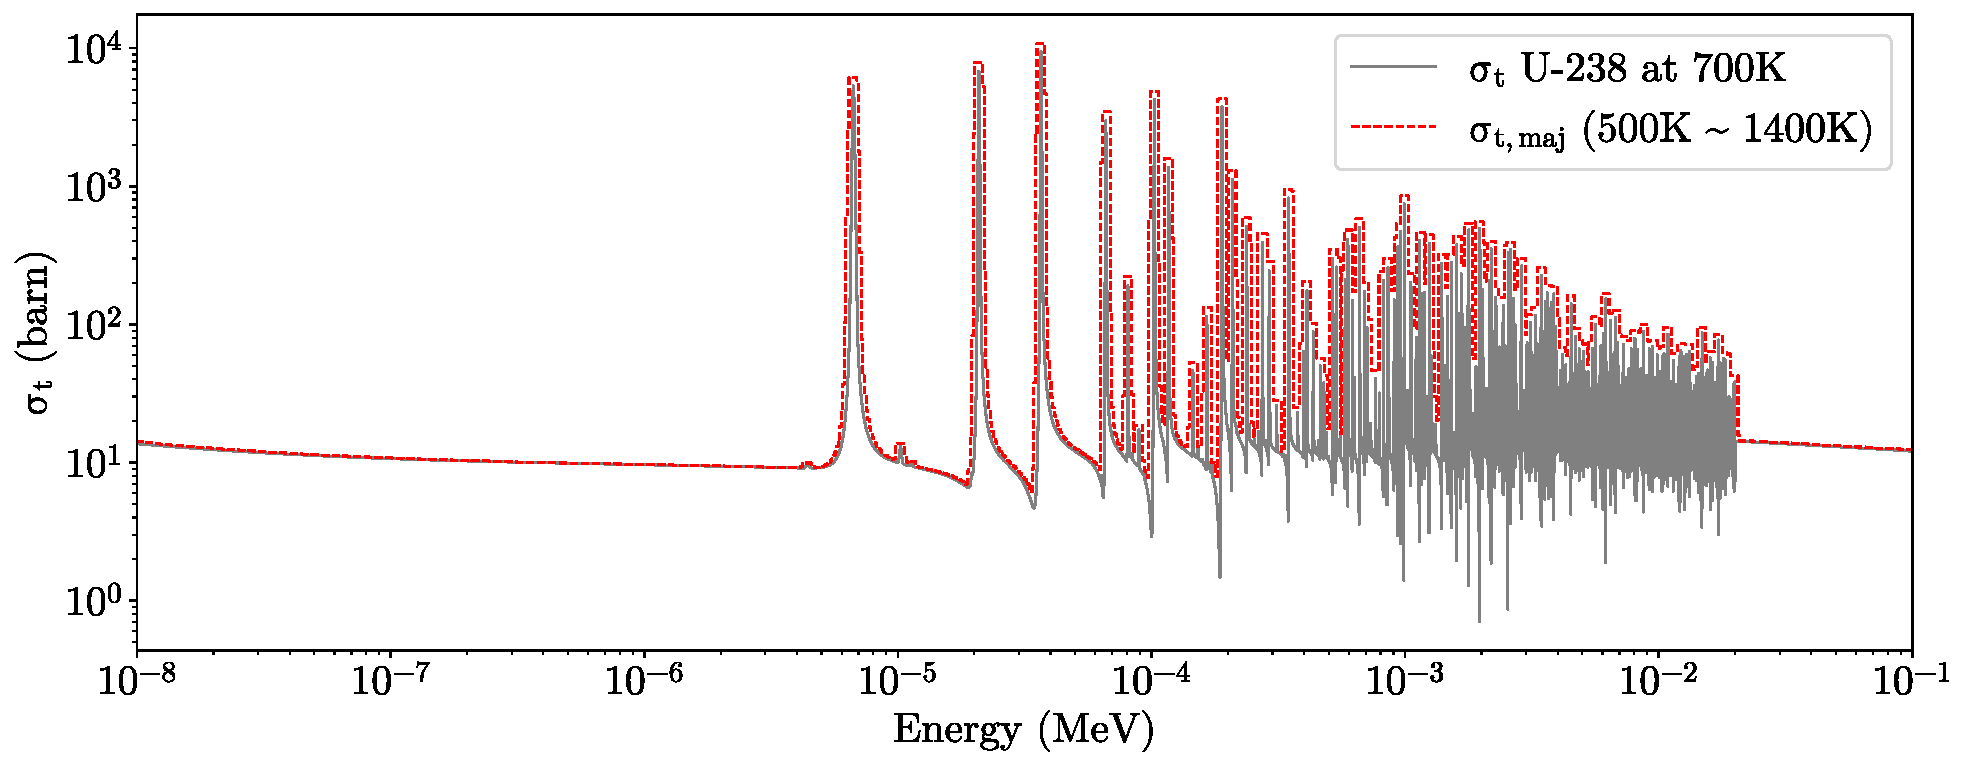
\includegraphics[width=0.95\textwidth]{figs/maj.pdf}
    \caption[Comparison of majorant microscopic XS of U-238]{Comparison of majorant microscopic XS of U-238 for temperature ranges 500 K - 1400 K and point-wise energy grid of U-238 at 700 K}
    \label{fig_2}
\end{figure}
\begin{figure}
    \centering
    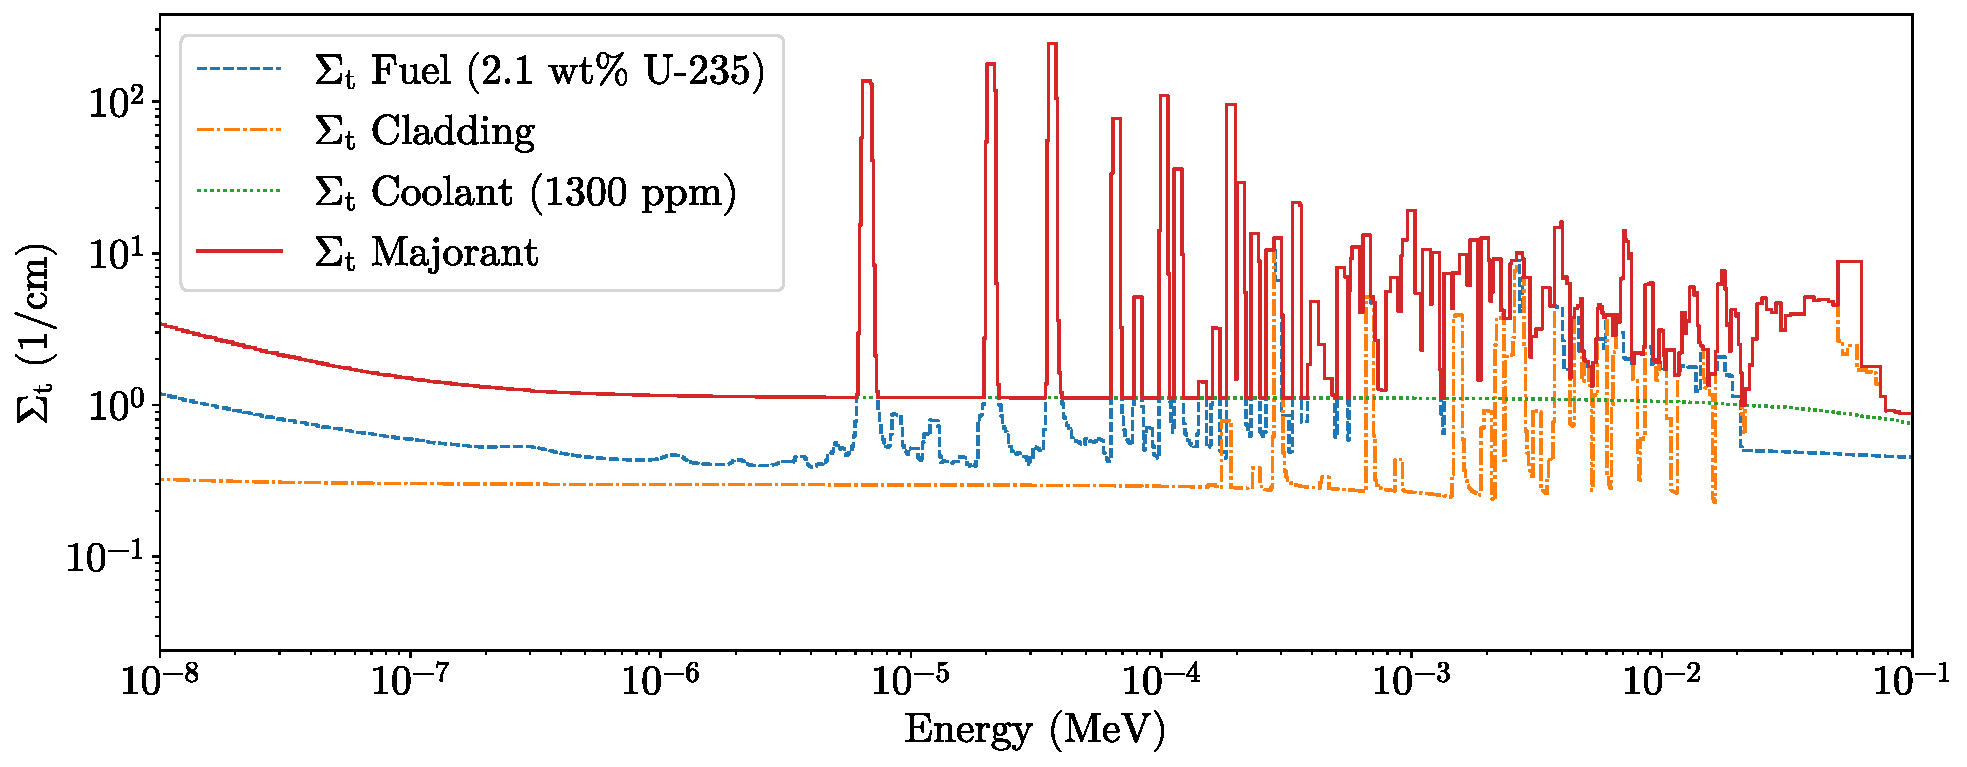
\includegraphics[width=0.95\textwidth]{figs/maj_mat.pdf}
    \caption[Comparison of majorant macroscopic XS]{Comparison of majorant macroscopic XS and material-wise majorant macroscopic XS.}
    \label{fig_3}
\end{figure}

\subsection{Calculation Flow} \label{sec25}

The simplified calculation flow of MC coupled multi-physics with spatially continuous material properties is illustrated in Figure \ref{fig_4}. The simulation begins with the evaluation of the majorant microscopic cross section, followed by the majorant macroscopic cross section. Particle delta-tracking in a continuous medium proceeds for several cycles, during which FET coefficients are tallied using Eq. \ref{eq5}. After several cycles of particle transport, a thermal-hydraulics (TH) update is conducted. If necessary, updates on critical boron concentration (CBC) and Xenon distribution are also performed.

During the TH update procedure, the two-dimensional nearly continuous power distribution is estimated using the truncated summation of Eq. \ref{eq1}, with coefficients tallied from previous cycles of particle tracking. This power distribution is then utilized by the TH solver to update the temperatures of the fuel, cladding, and coolant, as well as the coolant density. These updated values — two-dimensional fuel temperatures and one-dimensional coolant and cladding temperatures, along with coolant density — are stored for each fuel pin and serve as interpolation points during subsequent particle transport cycles. Similarly, these distributions of material properties are also nearly continuous. If equilibrium xenon feedback is active, a comparable process is used to reconstruct the two-dimensional xenon distribution across the fuel pin. It is worth noting that during inactive cycles, the tallied FET coefficients are discarded at every TH update. However, during active cycles, these FET coefficients are accumulated.

In previous work by Ellis \cite{ellis, ellis_2016}, functional expansion was used to represent the continuity of material properties, such as fuel temperature and coolant density. However, using interpolation instead of functional expansion to determine material properties at any point offers a key advantage: it requires fewer arithmetic operations than polynomial reconstruction, thus enhancing particle tracking efficiency.

The calculation of macroscopic cross sections for particle tracking in spatially continuous materials differs from conventional methods, where each cell is assigned unique material properties. In the case of particle tracking within spatially continuous materials, when a neutron is in the fuel pellet, a two-dimensional interpolation in both the axial and radial directions is employed to determine the fuel temperature at given spatial point. When a neutron in the coolant, a one-dimensional interpolation in the axial direction determines the temperature and density at given spatial point, followed by updates to the nuclide densities in the coolant. Lastly, for a neutron in the cladding, a one-dimensional interpolation in the axial direction determines the cladding temperature. After these temperatures and densities are determined, the microscopic cross section for a given energy and temperature is calculated for all nuclides within the material. Finally, the macroscopic cross section at the neutron's location is computed. These processes are summarized in Figure \ref{fig_5}.

\begin{figure}
    \centering
    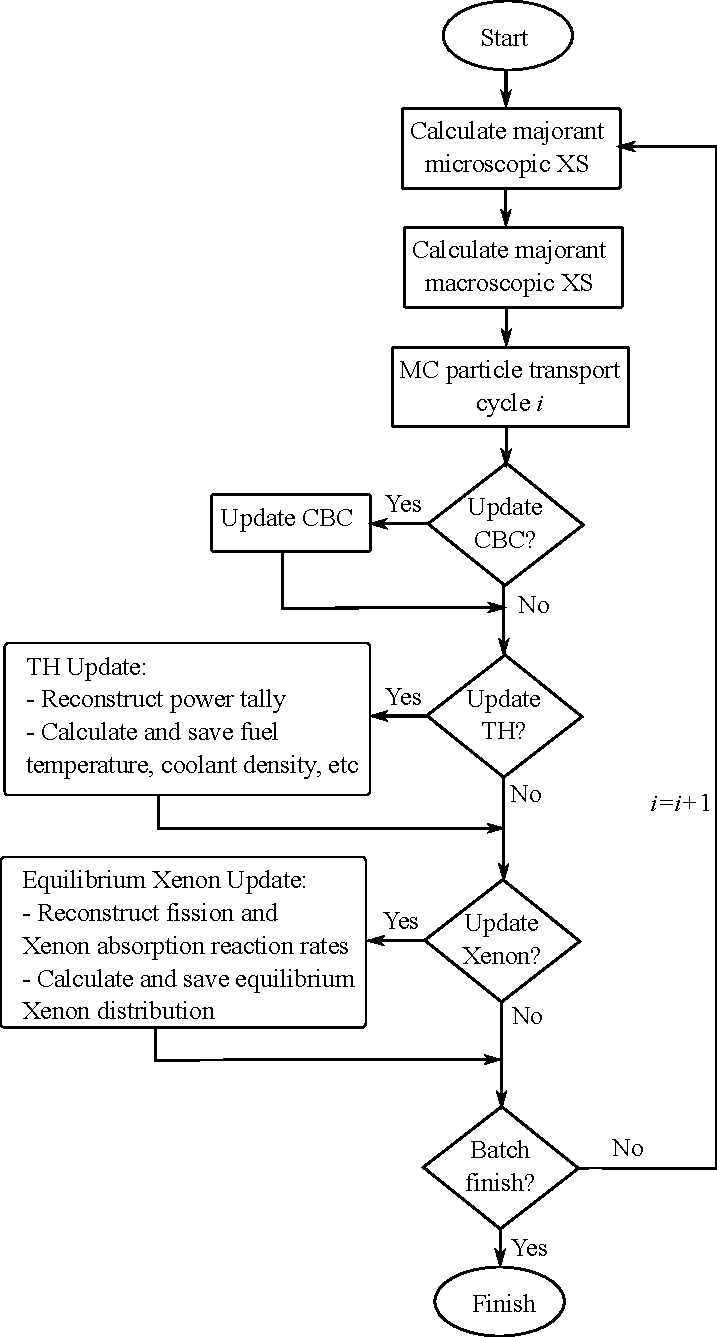
\includegraphics[width=0.65\textwidth]{figs/calc_flow_1.pdf}
    \caption{Calculation flow of the proposed framework.}
       \label{fig_4}
\end{figure}
\begin{figure}
    \centering
    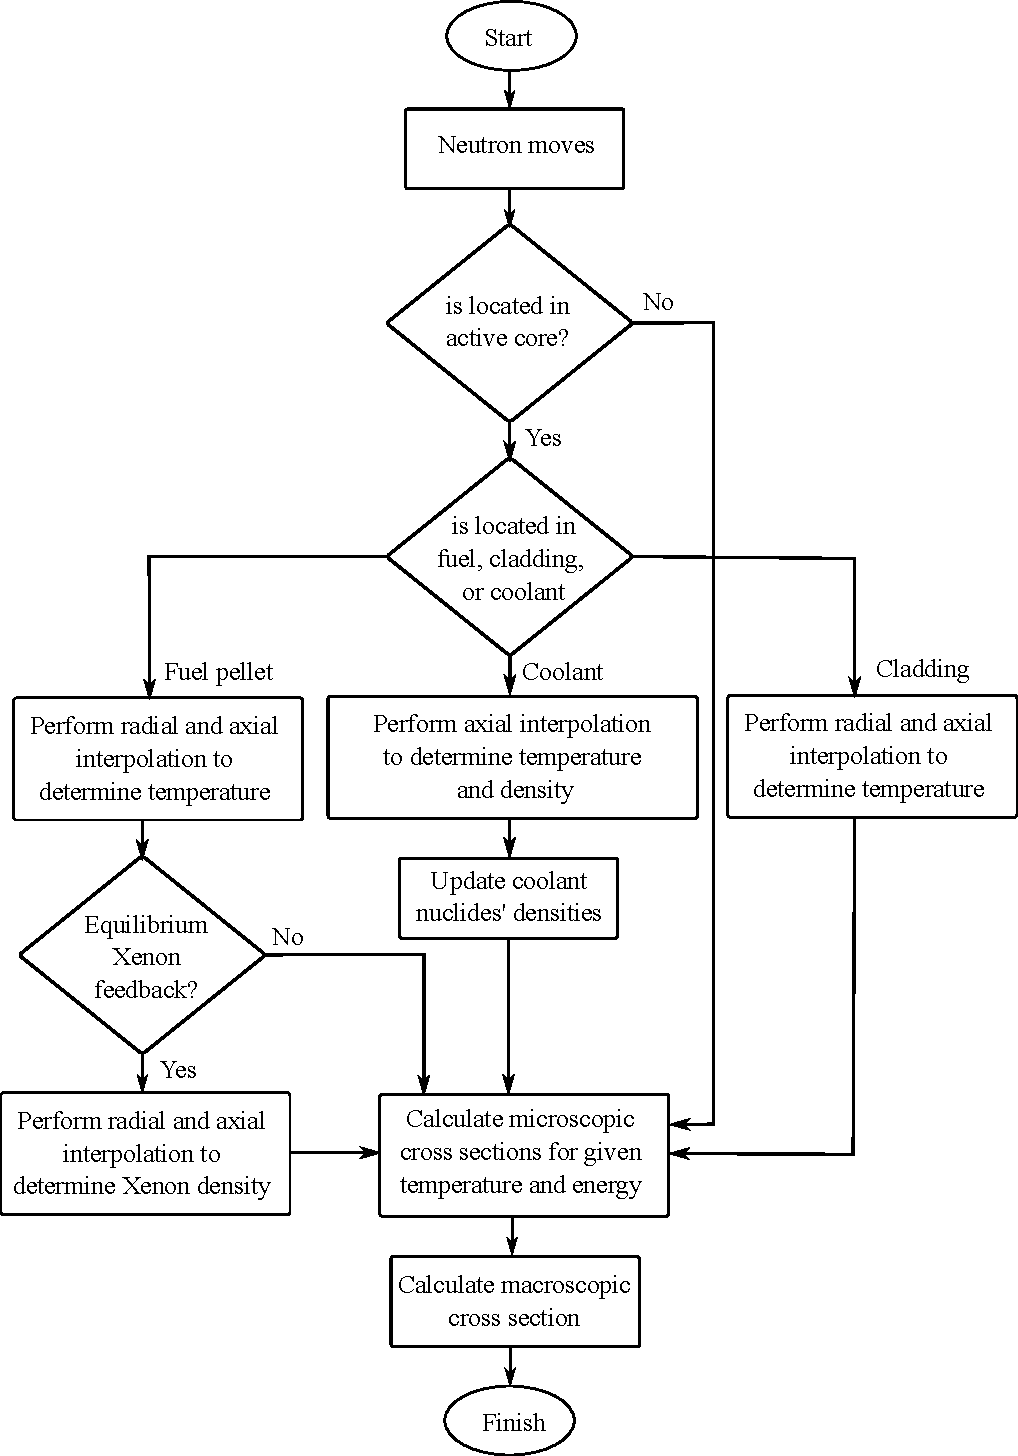
\includegraphics[width=0.85\textwidth]{figs/calc_flow_2.pdf}
    \caption[Calculation flow to calculate macroscopic cross section]{Calculation flow to calculate macroscopic cross section in spatially continuous particle transport.}
       \label{fig_5}
\end{figure}